Large feedback control gains are required if:
\begin{enumerate}
	\item There exist almost cancelling pole-zero pairs in the open loop TF, making the system almost uncontrollable.
\begin{center}
	\resizebox{300pt}{!}{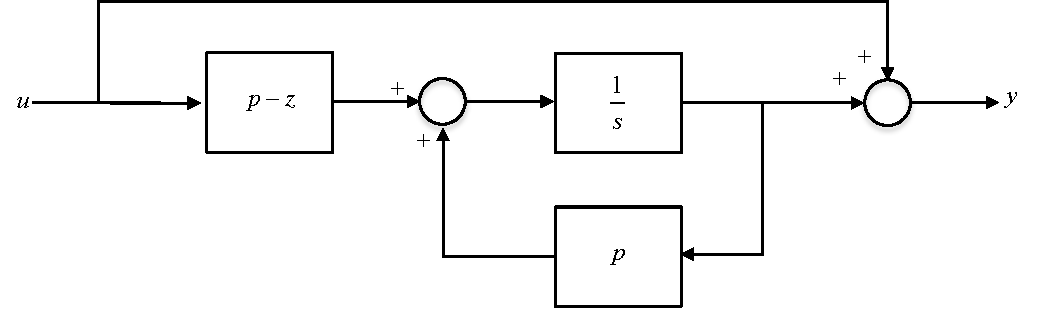
\includegraphics{pictures/zeroloc.pdf}}
\end{center}
	(Notice that in this condition the input $u$ is almost disconnected from the integrator for the state.)
	\item One tries to move the poles a long way, ($|p-p_c|$ large). 
	
	This imposes a practical limit on how arbitrarily 
	the poles can be placed. You cannot make a slow system fast without using large gains requiring powerful, 
	expensive actuators to force the plant response. Indeed, excessively large forces may destroy the plant.
\end{enumerate}

\endinput

%%% Local Variables: 
%%% mode: latex
%%% TeX-master: "notes"
%%% End: